\section{Romain et le sapin de Noël (3 points)}

%\begin{multicols}{2}
	Romain a un mini sapin de Noël qui décoré de trois guirlandes lumineuses alimentées par une pile. Il mesure les intensités sans le circuit mais son ampèremètre tombe en panne avant qu'il n'ait pu mesurer l'intensité $I_3$ qui traverse la guirlande bleue.
	
	\begin{questions}
		\question Comment peut-il faire pour déterminer $I_3$ sans la mesurer ? 
		
		\begin{solution}
			Il s'agit d'un montage en dérivation, donc l'intensité du courant dans la branche principale est égale à la somme des intensités dans les branches dérivées, donc :
			\begin{eqnarray*}
				I_1 &=& I_2 + I_3 + I_4 \\
				I_3 &=& I_1 - (I_2 + I_4) \\
			\end{eqnarray*}
		\vspace*{-0.8cm}
		\end{solution}
	
		\question Quelle valeur trouvera-t-il ?
		
		\begin{solution}
			On a donc :			
			\vspace*{-0.8cm}
			\begin{eqnarray*}			
				I_3 &=& I_1 - (I_2 + I_4)\\
				I_3 &=& 450 - (250 + 125)\\
				I_3 &=& 125\\
			\end{eqnarray*}		
		
		\vspace*{-0.8cm}			
			La guirlande bleue est donc traversée par une intensité $I_3$ égale à $125 mA$.
		\end{solution}
	\end{questions}

\textbf{Données : } $I_1 = 450 mA$, $I_2 = 250 mA$, $I_4 = 125 mA$

\begin{center}
	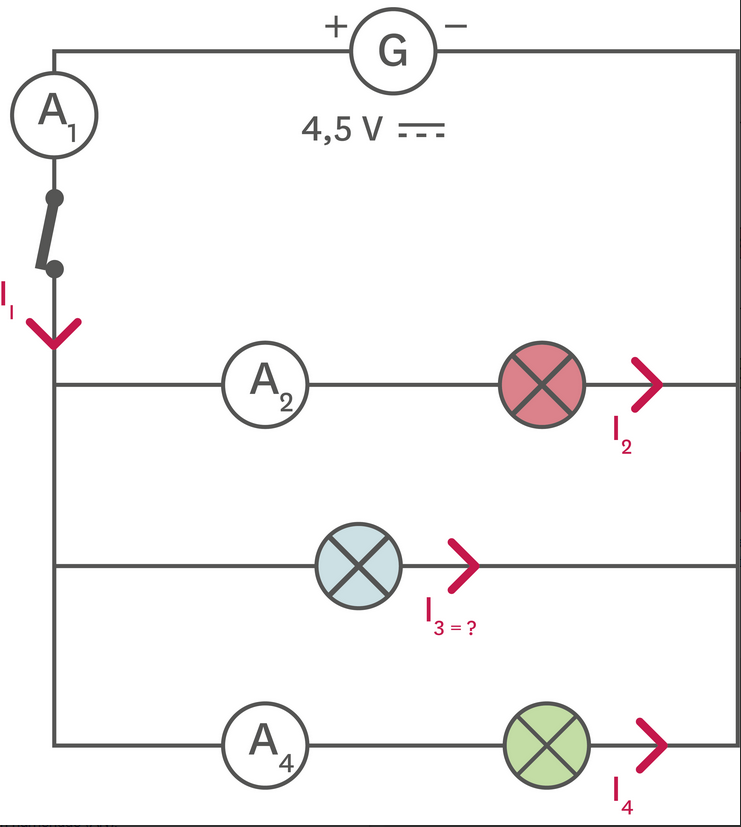
\includegraphics[scale=0.5]{img/sapin}
\end{center}
%\end{multicols}